\section{Bevölkerungsdichten der Landkreise}
Zuallererst folgen die genutzten Daten, welche nichts mit Corona zutun haben: Die Landkreise und ihre Bevölkerungsdichte. Die Bevölkerungsdichte wird aus der Bevölkerungszahl und der Fläche des Landkreises berechnet, welche von der API bereitgestellt werden \todo{adäquate Verlinkung auf API}.

In Abbildung \autoref{fig:distribution_pop_density_counties} sind die Bevölkerungsdichten der einzelnen Landkreise dargestellt. Auf der linken Seite befindet sich die Verteilung und auf der rechten Seite die räumliche Anordnung.
Die Bezirke Berlins sind einzeln gelistet, daher entsprechen die sechs höchsten Bevölkerungsdichten den Berliner Bezirken  Friedrichshain-Kreuzberg, Mitte, Neukölln, Tempelhof-Schöneberg, Lichtenberg, Charlottenburg-Wilmersdorf, obwohl die Bevölkerungsdichte des gesamten Berliner Stadtkreises niedriger ist als die Bevölkerungsdichte Münchens (in dieser Auflistung Platz 7, ohne Berliner Bezirke Platz 1).

\begin{figure}[H]
    \centering
    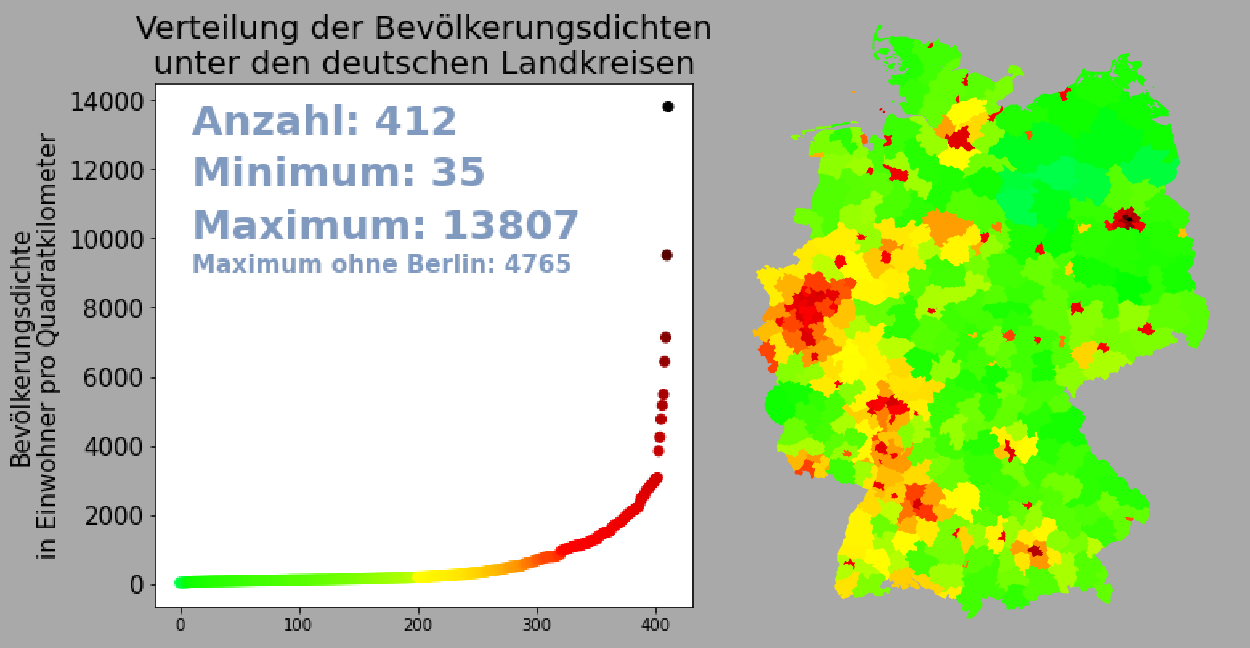
\includegraphics[width = 0.95\textwidth]{figures/Vorgehensweise/population_density_counties_Distribution_and_map.png}
    \caption{Verteilung der Bevölkerungsdichten unter den deutschen Landkreisen.}
    \label{fig:distribution_pop_density_counties}
\end{figure}

\todo{klarstellen, das die Landkreise nicht den Landkreisen entsprechen (Berlin ist aufgeteilt) Aus Wikipedia "Landkreis": In Deutschland gibt es 294 Landkreise. Zusammen mit den 106 kreisfreien Städten bilden sie die insgesamt 400 Gebietskörperschaften auf Kreisebene. Wir haben 412.}
In Abbildung 


\begin{figure}[H]
    \centering
    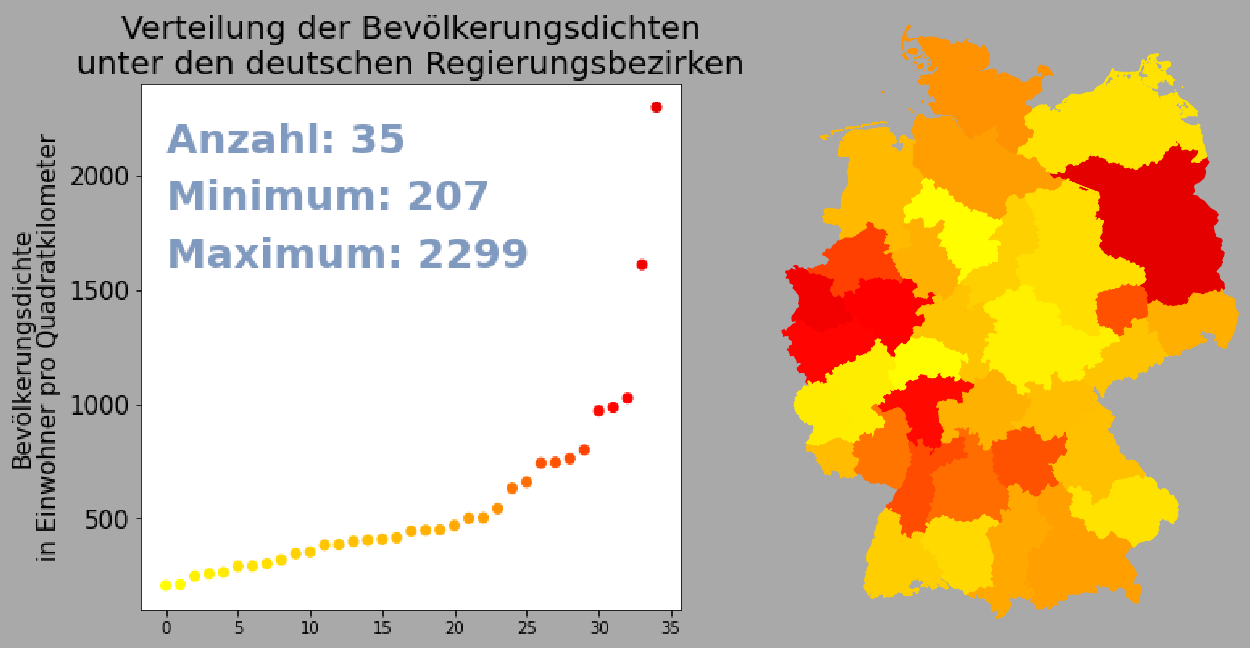
\includegraphics[width = 0.95\textwidth]{figures/Vorgehensweise/population_density_districts_Distribution_and_map.png}
    \caption{Verteilung der Bevölkerungsdichten unter den deutschen Regierungsbezirken. Die Skalierung entspricht der Farbgebung in \autoref{fig:distribution_pop_density_counties}.}
    \label{fig:distribution_pop_density_districts}
\end{figure}

Klar zu erkennen sind die Stadtkreise in Abbildung \ref{fig:distribution_pop_density_counties}: Sie weisen eine hohe Bevölkerungsdichte auf und sind in der Regel von weniger stark bevölkerten Landkreisen umgeben.

\section{Bevölkerungsdichte der Regierungsbezirke}
Teilt man die Landkreise nach den ersten beiden Kennzahlen des Landkreises, die des Bundeslandes und die des aktuellen (teils auch vergangenen) Regierungsbezirks, ein, ergibt sich für die Bevölkerungsdichte das in \autoref{fig:distribution_pop_density_districts} dargestellte Bild.